\subsection{Inverting Amplifier:}

Setting the {\itshape waveform generator} in a sinusoidal signal with a frequency of 1 KHz and 1 $V_{pp}$ we connect the positive terminal of the {\itshape generator} to the $V_{i}$ input of the circuit of Figure 3.1.0 ( is the one on the left side of the 1 K$\Omega$ resistor ) and the negative terminal to the common ground. Then, once the respectively sources in the terminals 7 and 4 were connected, we turned on the {\itshape generator} and the voltage sources, thus, connecting the channel 1 of the oscilloscope in the input $V_{i}$ and the channel 2 in the output $V_{o}$ we registered the waveform in Figure 3.1.1. \hfill \break

\begin{figure}[H]
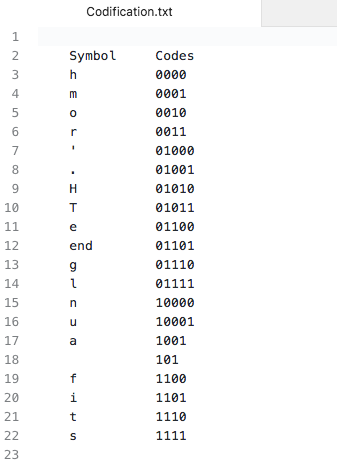
\includegraphics[width = 8cm, height = 5cm]{c1.png}
\centering \linebreak \linebreak Figure 3.1.0: Inverting amplifier circuit.
\end{figure} \hfill

The oscilloscope has another way to display the waveform, setting the device in its mode XY we will be able to visualize the {\bfseries Transfer Function} as in Figure 3.1.2. \hfill \break

\begin{multicols}{2}
\begin{figure}[H]
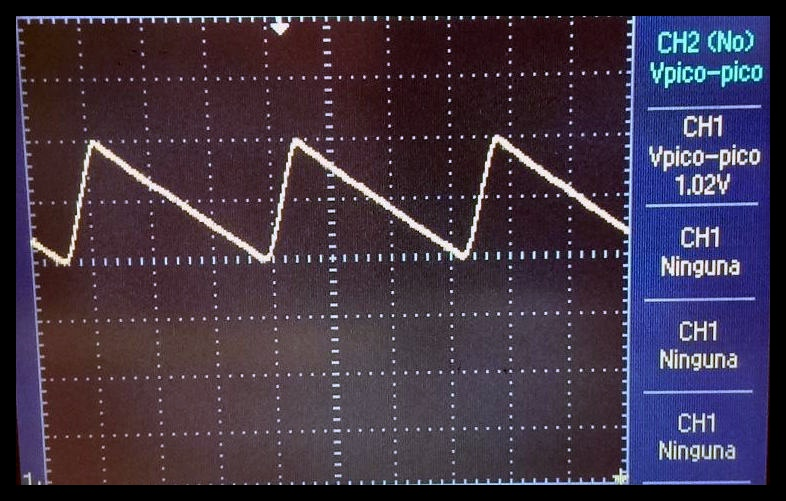
\includegraphics[width = 8cm, height = 4.5cm]{o1.jpg}
\centering \linebreak \linebreak Figure 3.1.1: Input and output waveform.
\end{figure}

\begin{figure}[H]
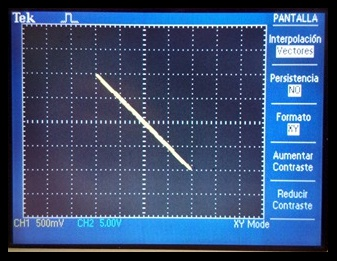
\includegraphics[width = 8cm, height = 4.5cm]{tf1.jpg}
\centering \linebreak \linebreak Figure 3.1.2: Transfer Function.
\end{figure}
\end{multicols} \hfill

{\bfseries\itshape\color{carmine}{Observation:}} {\itshape\color{carmine}{The yellow waveform corresponds to the channel 1 and the blue waveform to channel 2 for Figure 3.1.1.}} \hfill \break

Finally, we capture the gain and the input and output voltage values in Table 1: \hfill \break

\begin{center}
\begin{tabular}[.5cm]{c c c}
\toprule
\toprule
\hspace{60pt} $V_{i}$ \hspace{60pt} & \hspace{60pt} $V_{o}$ \hspace{60pt} & \hspace{60pt}  {\bfseries Gain} \hspace{60pt}  \\
\midrule
\midrule
1 $V_{pp}$ & 10.12 $V_{pp}$ & 10 \\
\bottomrule
\linebreak
\end{tabular}
\linebreak Table 1: Gain of Inverting Amplifier.
\end{center}

\pagebreak